\chapter{Sistema Mecânico}

O robô utilizado no projeto é o mesmo robô construído durante o projeto \textbf{Robô Explorador de Labirintos 2D} \cite{Robo2d} desta mesma disciplina.

No projeto original o robô era utilizado para explorar e solucionar labirintos em duas dimensões feitos através de trilhas pretas em um chão branco, utilizado emissores e sensores de luz infravermelha para identificar a pista. 

Todo o projeto mecânico foi reutilizado neste trabalho, incluindo rodas, caixa de redução e chassi. Foram reutilizados também o sistema de alimentação e a uma placa \textit{Arduíno Duemilanove}; o conjunto de sensores do robô original foi substituído por uma câmera \textit{CMUCam3}.

\section{Projeto Mecânico}

O diagrama do projeto físico do robô é apresentado na Figura \ref{int_fig01}.

\begin{figure}[h!]
    \center
    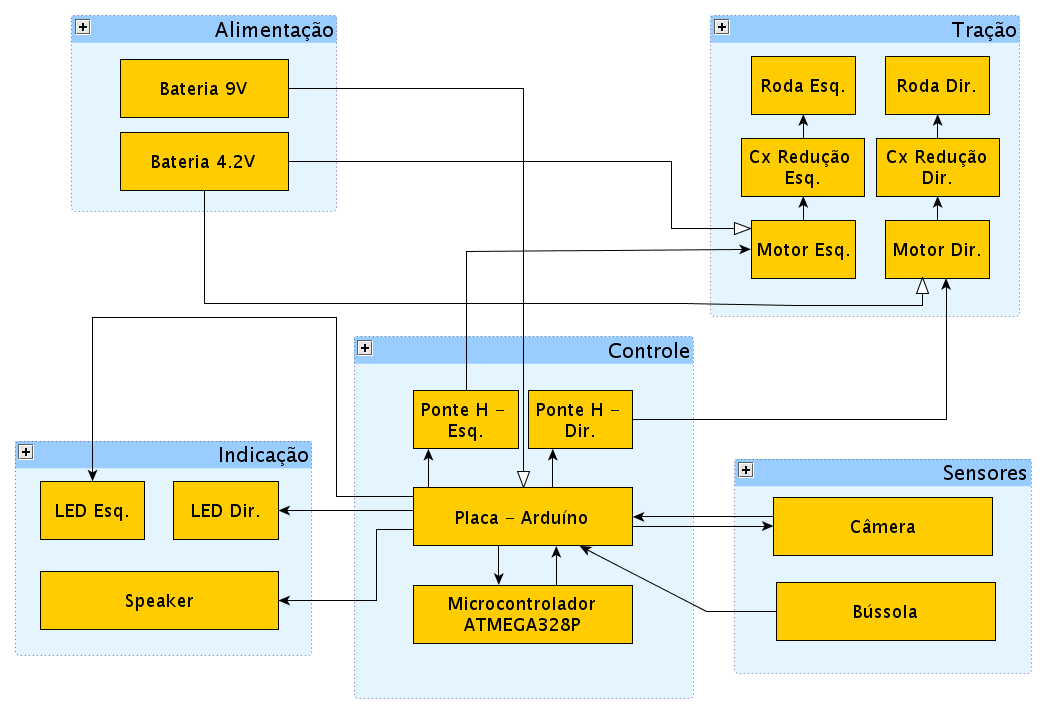
\includegraphics[scale=0.35]{imagens/robo_geral.png}
    \caption{Diagrama do Robô}
    \label{int_fig01}
\end{figure}

\subsection{Sistema de Alimentação}

Conjunto de baterias utilizadas como alimentação do robô.

\subsubsection{Bateria de 9V}
Utilizada para alimentação do \textit{Arduíno Duemilanove}, uma bateria PP3.

\subsubsection{Bateria de 4,2V}
Usada na alimentação dos motores, bateria de câmera fotográfica digital.

\subsubsection{Bateria de 6V}
Usada na alimentação da CMUCam3, quatro pilhas AA em série.

\subsection{Sistema de Indicação}

LEDs e \textit{Speaker} usados para indicar as ações do robô.

\subsubsection{LEDs}
Usados para indicação dos estados do robô, detalhados na Tabela \ref{int_tbl01}

\subsubsection{Speaker}
Utilizado como indicador sonoro de estados específicos do sistema, como reconhecimento do objeto e início e fim da busca do mesmo.

\subsection{Sistema de Tração}

Para tração do robô foi construído um sistema baseado em um motor elétrico e duas rodas centrais.

\subsubsection{Motores}
Motor elétrico de corrente contínua \textit{Mabuchi FA-130RA} de 3V com rotação de 12300 rpm, ou 205 voltas por segundo \cite{Robo2d}

\subsubsection{Caixas de redução}
Acopladas ao motor e às rodas reduzem a rotação do motor para que seja possível acionar as rodas. Na configuração usada, a redução é de 344:1 \cite{Robo2d}.

\subsubsection{Rodas}
O robô utiliza duas rodas \textit{off-road} em seu centro e uma esfera com giro livre atrás para manter o equilíbrio.

Com a rotação de 205 voltas/segundo e a redução de 344:1, a roda completa 0,6 voltas por segundo.

\subsection{Sistema de Controle}

Sistema para controle da movimentação do robô.

\subsubsection{Ponte H} 

A Ponte H é um circuito que permite a um microcontrolador acionar um motor de corrente contínua. Por questões eletrônicas \cite{Robo2d}, o circuito utilizado no projeto foi construído a partir de componentes discretos.

\subsubsection{Arduíno Duemilanove}

Placa \textit{Arduíno} utilizada no projeto anterior e reutilizada no projeto atual. Faz o interfaceamento dos diversos sistemas do projeto, \textit{i.e.}, recebe as decisões tomadas pelo Sistema de Navegação, embarcado na câmera, e aciona os motores para que o robô as execute. Seu funcionamento é detalhado na seção \ref{sec_arduino}.

\subsubsection{Microcontrolador ATMEGA328P}

Microcontolador presente da \textit{Arduíno Duemilanove}, os códigos construídos para controle do robô (Seção \ref{sec_soft_controle}) serão executados por ele.

\subsection{Sensores}

São apresentados na seção \ref{sec_sensores}.

\subsubsection{Câmera}

Ver seção \ref{sec_camera}.

\subsubsection{Bússola}

Ver seção \ref{sec_bussola}.

\section{Plataforma Arduíno}
\label{sec_arduino}

Arduíno é uma plataforma \textit{open-source} para prototipagem eletrônica que busca facilitar a construção de sistemas onde haja interação com objetos e o ambiente. \cite{arduino1}

Para o projeto \textbf{Robô Explorador de Labirintos 2D} foi utilizado uma placa \textit{Arduíno Duemilanove} que foi reutilizada no trabalho atual.

Dentro do projeto, o \textit{Arduíno} exerce um papel central de receber, via comunicação serial, as decisões tomadas pelo Sistema de Exploração, embarcado na câmera, e atuar sobre os motores através da Ponte H. Além disso, ele recebe o sinal lido através da bússola e aciona os dispositivos de indicação. Esse processo é representado na Figura \ref{int_fig02}.

\begin{figure}[h!]
    \center
    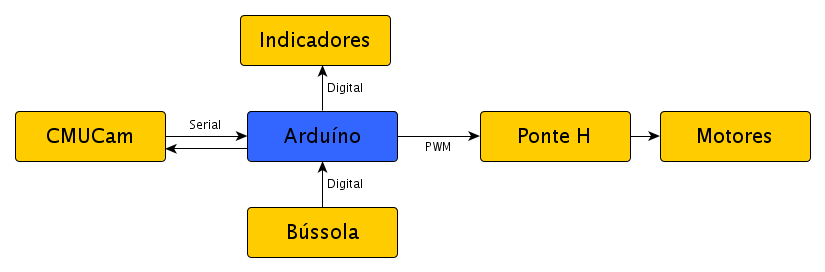
\includegraphics[scale=0.5]{imagens/processo_arduino.png}
    \caption{Processo de Comunicação - Arduíno}
    \label{int_fig02}
\end{figure}

O \textit{Arduíno Duemilanove} possui um microprocessador \textit{ATMEGA328P}, sua programação pode ser feita utilizando a linguagem de programação própria, baseada em \textit{Wiring} \cite{arduino1}. No entanto, é possível utilizar \textit{C++} para construir bibliotecas próprias utilizando também as bibliotecas já prontas do \textit{Arduíno}, e essa foi a opção feita pela equipe. O software de controle é detalhado na Seção \ref{sec_soft_controle}.

Para o interfaceamento com os diversos módulos do sistema, o \textit{Arduíno Duemilanove} possui 14 pinos de comunicação digital \cite{arduino2}, a configuração e utilização desses pinos está resumida na Tabela \ref{int_tbl02}.

\begin{table}[h!]
    \centering
    \begin{tabular}{|c|c|c|c|} \hline
        \textbf{Pino} & \textbf{Sentido do Sinal} & \textbf{Tipo de Comunicação} & \textbf{Função} \\ \hline
        00 & (RX) & Serial & Comunicação Câmera \\ \hline
        01 & (TX) & Serial & Comunicaçao Câmera \\ \hline
        02 & Entrada & Digital TTL & Bússola - Pino 1 \\ \hline
        03 & Entrada & Digital TTL & Bússola - Pino 4 \\ \hline
        04 & Saída & Digital TTL &LED Direito \\ \hline
        05 & Saída & Sinal PWM & Motor Esquerdo - Pino 2 \\ \hline
        06 & Saída & Sinal PWM & Motor Esquerdo - Pino 1 \\ \hline
        07 & Entrada & Digital TTL & Bússola - Pino 3 \\ \hline
        08 & Entrada & Digital TTL & Bússola - Pino 2 \\ \hline
        09 & Saída & Digital TTL & \textit{Speaker} \\ \hline
        10 & Saída & Sinal PWM & Motor Direito - Pino 2 \\ \hline
        11 & Saída & Sinal PWM & Motor Direito - Pino 1 \\ \hline
        12 & Saída & Digital TTL & LED Esquerdo \\ \hline
        13 & - & - & \textit{Não utilizado} \\ \hline
    \end{tabular}
    \caption{Pinos da placa \textit{Arduíno Duemilanove}}
    \label{int_tbl02}
\end{table}

\subsection{Comunicação com Indicadores}

Os indicadores do robô são os LEDs, esquerdo e direito, e o \textit{Speaker}. 

Os estados possíveis dos LEDs são aceso ou apagado, como visto na Tabela \ref{int_tbl01}. Para produzir os dois estados, é utilizada uma comunicação digital TTL, em que um sinal baixo (\textit{LOW}) produzirá o estado apagado e o sinal alto (\textit{HIGH}) irá deixar o LED aceso.

\begin{table}[h!]
    \centering
    \begin{tabular}{|c|c|c|} \hline
        \textbf{Estado} & \textbf{LED Esquerdo} & \textbf{LED Direito} \\ \hline
        Parado & Apagado & Apagado \\ \hline
        Andando para frente & Aceso & Apagado \\ \hline
        Virando para esquerda & Aceso & Apagado \\ \hline
        Virando para direita & Apagado & Aceso \\ \hline
    \end{tabular}
    \caption{Sistema de Indicação}
    \label{int_tbl01}
\end{table}

O LED Direito é ligado no pino 04 e o Esquerdo no 12.

Para o \textit{Speaker} é gerado um sinal com \textit{duty-cycle} de 50\% numa frequência especificada através da função \textit{tone} presente na biblioteca básica do \textit{Arduíno}.

O Speaker é ligado ao \textit{Arduíno} através do pino 09.

\subsection{Comunicação com Bússola}

A bússola utilizada pela equipe é a \textit{Dinsmore Sensor Modelo \#1490}, uma bússola digital com precisão de 45 graus, ou oito estados \cite{bussola}.

A \textit{Dinsmore \#1490} gera quatro sinais digitais TTL, a combinação desses sinais fornece a orientação lida pela bússola.

Os quatro sinais são ligados nos pinos 02, 03, 07 e 08 do \textit{Arduíno}.

Para funcionamento detalhado da bússola, ver seção \ref{sec_bussola}.

\subsection{Acionamento dos Motores}
\label{sec_com_motores}

Para acionamento dos motores, são utilizadas Pontes H, circuitos eletrônicos que permitem o acionamento por parte de um microcontrolador de um motor de corrente contínua em qualquer sentido de rotação. Por não ser objeto de estudo deste trabalho, seu funcionamento e a construção do circuito utilizado no robô não será explicitado, maiores informações podem ser encontradas em \cite{Robo2d} e \cite{ponteh}. 

A Ponte H, por sua vez, é acionada através de um sinal PWM - \textit{Pulse Width Modulation}. A modulação por largura de pulso é uma técnica usada para obter resultados analógicos com um sinal digital \cite{arduino3}. Uma onda quadrada é gerada, mudando o período em que essa onda está em ALTO (\textit{duty cycle}) é possível obter níveis médios de tensão diferentes. Assim, por exemplo, uma onda sempre em BAIXO, produrizá 0 V de nível médio de tensão, uma onda sempre em ALTO, 5 V; e uma onda 50\% do tempo em ALTO, 2,5 V. Esses diferentes níveis de tensão produzirão diferentes velocidades nos motores.

O \textit{Arduíno} possui portas que implementam o PWM, para utilizá-las é necessário usar a função \textit{analogWrite} que recebe como parâmetro um inteiro entre 0 e 255. Esse valor irá definir o tempo em que o sinal gerado ficará em ALTO.

Neste projeto, na maior parte dos movimentos, a velocidade do robô é constante, então foi definido experimentalmente o valor 127 para parâmetro da função \textit{analogWrite}, que produzirá um \textit{duty-cycle} de 50\%, e metade da velocidade do robô. Nos movimentos de correção do alinhamento do robô, esse valor é alterado para 40 ou 60\%.

Para cada Ponte H são gerados dois sinais que irão acionar os motores para frente ou para trás. Quando o sinal 1 é ALTO e o 2 é BAIXO, o motor gira num sentido, para frente, por exemplo; sinal 1 em BAIXO e sinal 2 em ALTO, ele gira no sentido inverto, para trás; esses sinais em função da ação executada pela robô são apresentados na tabela \ref{int_tbl03}.

\begin{table}[h!]
    \centering
    \begin{tabular}{|c|c|c|} \hline
        \textbf{Ação} & \textbf{Motor Esquerdo} & \textbf{Motor Direito} \\ \hline
        Parado & Desligado & Desligado \\ \hline
        Para frente & Frente & Frente \\ \hline
        Para trás & Trás & Trás \\ \hline
        Virando esquerda & Frente & Desligado \\ \hline
        Virando direita & Desligado & Frente \\ \hline
        Rotacionando esquerda & Frente & Trás \\ \hline
        Rotacionando direita & Trás & Frente \\ \hline
    \end{tabular}
    \caption{Acionamento dos Motores}
    \label{int_tbl03}
\end{table}

\subsection{Comunicação com CMUCam}

As decisões de movimentação são tomadas na aplicação que roda no microprocessador da câmera, no entanto quem aciona os motores e de fato produz o movimento é a aplicação executada no \textit{Arduíno}, por isso a necessidade de comunicação entre os dois dispositivos.

Esse interfaceamento entre o \textit{Arduíno} e a \textit{CMUCam} é feito através de comunicação serial assíncrona \textit{full-duplex}.

Por comunicação serial, entende-se aquela em que os \textit{bits} são enviados em \textit{fila} por um mesmo canal de comunicação. Por ser assíncrona, não há necessidade sincronismo de tempo entre os dois dispositivos envolvidos na comunicação, a própria mensagem irá definir o sinal de sincronismo. Como há necessidade de envio de mensagens da câmera para o \textit{Arduíno} e do \textit{Arduíno} para a câmera, a comunicação precisa ser \textit{full-duplex}, isso é, trafegar nos dois sentidos.

Para cada troca de mensagem será enviado um byte entre os dispositivos.

As mensagens que trafegarão da \textit{CMUCam} para o \textit{Arduíno} conterão comandos de ação para o robô, andar para frente ou para trás, rotacionar para a esquerda ou para a direita, parar o robô ou ainda corrigir o movimento do robô para determinado lado \footnote{Quando o movimento do robõ for por demais irregular e ele não conseguir seguir uma linha reta.}. E a câmera pode ainda requisitar ao \textit{Arduíno} a leitura de informação da bússola, nesse momento o \textit{Arduíno} envia para ela a informação do sensor.

Foram definidas constantes que serão enviadas de um dispositivo para o outro, apresentadas na Tabela \ref{int_tbl04}.

\begin{table}[htb!]
    \centering
    \begin{tabular}{|c|c|l|} \hline
        \textbf{Valor} & \textbf{Constante} & \textbf{Signficado} \\ \hline

        \multicolumn{3}{|c|}{\textit{Operações para o robô - Camêra-Arduíno}} \\ \hline
        1 & FORWARD & Movimenta robô para frente \\ \hline
        2 & BACKWARD & Movimenta robô para trás \\ \hline
        3 & SPINLEFT & Rotaciona robô para esquerda \\ \hline
        4 & SPINRIGHT & Rotaciona robô para direita \\ \hline
        5 & STOP & Pára robô \\ \hline
        6 & COMPASS & Executa leitura da bússola\\ \hline
        7 & ADJUSTLEFT & Corrige movimento do robô para esquerda \\ \hline
        8 & ADJUSTRIGHT & Corrige movimento do robô para direita \\ \hline
            
        \multicolumn{3}{|c|}{\textit{Leituras da bússola - Arduíno-Câmera}} \\ \hline
        1 & NORTH & Norte \\ \hline
        2 & NORTHEAST & Nordeste \\ \hline
        3 & EAST & Leste \\ \hline
        4 & SOUTHEAST & Sudeste \\ \hline
        5 & SOUTH & Sul \\ \hline
        6 & SOUTHWEST & Sudoeste \\ \hline
        7 & WEST & Oeste \\ \hline
        8 & NORTHWEST & Noroeste \\ \hline
    \end{tabular}
    \caption{Comunicação Arduíno-Câmera}
    \label{int_tbl04}

\end{table}


\section{Software de Controle}
\label{sec_soft_controle}

O Sistema de Controle executado no \textit{Arduíno} é responsável por receber e interpretar os comandos enviados pela \textit{CMUCam3} e atuar sobre os motores do robô produzindo o movimento necessário. Para executar essa tarefa, a equipe desenvolveu uma biblioteca orientada a objetos em \textit{C++}, cujo diagrama básico é apresentado na figura \ref{int_fig03}.

A ideia de construir a classe se baseia em representar em código a maneira como a equipe enxerga a função do \textit{Arduíno} e tentar encapsular as funções em classes que devem então ser apenas instanciadas, facilitando a programação, já que operações por vezes complexas são convertidas em operações elementares.

\begin{figure}[htb!]
    \center
    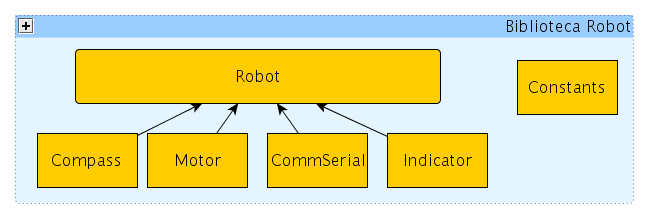
\includegraphics[scale=0.5]{imagens/diagrama_classe_robot.png}
    \caption{Diagrama - Biblioteca \textit{Robot}}
    \label{int_fig03}
\end{figure}

\subsection{Compass}

Classe responsável por fazer a leitura da bússola e decodificar o sinal lido, tendo como resposta apenas a constante que representa a direção cardeal lida.

\subsection{Motor}

Classe responsável por acionar os motores, recebe como parâmetro qual movimento deve ser feito e atua sobre os motores produzindo-o.

\subsection{CommSerial}

Classe para a comunicação com a \textit{CMUCam3}, possui um método de escrita e um de leitura apenas.

\subsection{Indicator}

Classe para produzir a representação necessária nos indicadores do robô.

\subsection{Robot}

Uma vez que todas as ações do robô estão definidas nas classes anteriormente citadas, a classe \textit{Robot} possui objetos das mesmas e sua tarefa é chamar as funções nos momentos adequados. 

No programa principal do \textit{Arduíno} há um objeto dessa classe que possui um método principal que funciona como um \textit{watchdog} para os comandos da \textit{CMUCam} através da classe \textit{CommSerial}, quando ele recebe um comando, dispara as funções das classes imediatamente abaixo.

\subsection{Constants}

Armazena as constantes definidas ao longo da biblioteca e não possui nenhum método. Armazena tanto as constantes de comunicação, Tabela \ref{int_tbl04}, quanto as constantes para acionamento dos motores, por exemplo.


